\chapter{Automorfismi delle superfici di Riemann semplicemente connesse}

Determiniamo ora i gruppi degli automorfismi delle superfici di Riemann semplicemente
connesse, che il teorema di Riemann dice essere $\mathbb{P}^1(\mathbb{C})$, $\mathbb{C}$, $D$.


\section{Automorfismi di $\mathbb{P}^1(\mathbb{C})=\hat{\mathbb{C}}$}

Identifico $\oc\bbC\isom\bbP_1(\bbC)$ con $\bbC\cup\{\infty\}$, attraverso la seguente mappa: $[z:1]\mapsto z, [1:0]\mapsto\infty$.

Considero $\phi\in\GL_2(\bbC)=\matrice abcd, ad-bc \neq 0$. $\phi$ è un isomorfismo lineare, dunque manda rette in rette, e si ha $\phi(z_0,z_1)=(az_0+bz_1,cz_0+dz_1)$. Questo isomorfismo, poichè manda rette in rette, induce un isomorfismo $\ot \phi$ a livello di $\oc\bbC$ tale che $\ot\phi[z_0,z_1]=[az_0+bz_1,cz_0+dz_1]$.

Sotto l'identificazione con $\bbC\cup\{\infty\}$, possiamo scrivere $\ot\phi(z)=\frac{az+b}{cz+d}$, dove si intende che $\ot\phi(\infty)=\frac{a}{c}$ e che $\frac{1}{0}=\infty$. Il gruppo degli isomorfismi di questa forma in $\oc \bbC$, con $ad\neq bc$, si chiama $\bbP\GL_2(\bbC)$, e si ha che $\bbP\GL_2(\bbC)\isom\quotient{\GL_2(\bbC)}{\{\lambda\Id\}}$.

Vogliamo dimostrare che $Aut( \hat{\mathbb{C}} )= \mathbb{P}GL_2 (\mathbb{C} )=\left\{z\mapsto \displaystyle{\frac{az+b}{cz+d}} \ ,\ \  ad\neq bc\right\}$

\begin{definizione}[Grado di una funzione razionale]
Si definisce grado di $\frac{p(x)}{q(x)}$ il massimo tra i gradi di $p(x)$ e $q(x)$.
Si può osservare che, come per i polinomi, il grado è il numero di controimmagini di ogni punto contate con molteplicità.
\end{definizione}

\begin{osservazione}
$\varphi \in Aut( \hat{\mathbb{C}} ) \Longrightarrow deg(\varphi )=1$, perché deve essere un omeomorfismo e quindi è iniettivo.
\end{osservazione}


\begin{lemma}
$G= \mathbb{P}GL_2 (\mathbb{C} )$ è triplamente transitivo, cioè date due terne
$(x_1 , x_2 , x_3 ) \in \hat{\mathbb{C}}^3$ e $(y_1 , y_2 , y_3 ) \in \hat{\mathbb{C}}^3$
con $x_i \neq x_j$ e $y_i \neq y_j$ se $i \neq j$, $\exists ! g \in G$ t.c. $g(x_i )=y_i$ per $i=1,2,3$.
\end{lemma}
\begin{proof}
Basta farlo per $(x_1 , x_2 , x_3 ) = (0,1,\infty )$ e $y_i \neq \infty$, a meno di comporre con qualche elemento di $G$.
Devo quindi trovare $a,b,c,d \in \mathbb{C}$ tali che:
$$
\left\{
\begin{array}{l}
\medskip
\displaystyle{\frac{0a+b}{0c+d}=\frac{b}{d}=y_1} \\
\medskip
\displaystyle{\frac{1a+b}{1c+d}=\frac{a+b}{c+d}=y_2} \\
\displaystyle{\frac{\infty a+b}{\infty c+d}=\frac{a}{c}=y_3}
\end{array}
\right.
$$
da cui sostituendo si ottiene $y_3 c + y_1 d=y_2 (c+d)$ e si vede che, se $y_i \neq y_j$ quando $i \neq j$, esistono $c$ e $d$ con $c+d \neq 0$ che risolvono l'equazione.

Resta quindi da mostrare l'unicità. Per farlo basta verificare che l'unico elemento di $G$ che fissa una data terna
(prendiamo ancora $(0,1,\infty )$) è l'identità. Imponiamo quindi che:
$$
\left\{
\begin{array}{l}
\medskip
\displaystyle{\frac{0a+b}{0c+d}=\frac{b}{d}=0} \\
\medskip
\displaystyle{\frac{1a+b}{1c+d}=\frac{a+b}{c+d}=1} \\
\displaystyle{\frac{\infty a+b}{\infty c+d}=\frac{a}{c}= \infty}
\end{array}
\right.
$$
da cui si ricava subito $a=d=1$, $b=0$ e $c=0$, cioè la trasformazione considerata è l'identità.
\end{proof}

\begin{esercizio}
I sottogruppi finiti di $\mathbb{P}GL_2 (\mathbb{C} )$ sono:
\begin{itemize}
\item Tutti i gruppi ciclici
\item Tutti gruppi diedrali
\item $S_4$ e $A_5$
\end{itemize}
\end{esercizio}


\begin{proposizione}
$Aut (\hat{\mathbb{C}} ) = G = \mathbb{P}GL_2 (\mathbb{C} )$
\end{proposizione}
\begin{proof}
Sia $\varphi \in Aut (\hat{\mathbb{C}} )$. Sappiamo già che $Aut (\hat{\mathbb{C}} ) \supseteq G$.
Quindi, essendo $G$ triplamente transitivo, possiamo assumere $\varphi( \infty ) = \infty$.
Ora osserivamo che, essendo $\varphi$ un automorfismo olomorfo, detto $D=D(0,1)$, $\varphi (D)$ conterrà
un certo disco $D_1$. Quindi $\varphi$ non può avere una sigolarità essenziale all'infinito poiché in tal caso,
per il teorema di Weierstrass, dovrebbe assumere valori densi in $\mathbb{C}$ in ogni intorno di $\infty$
e quindi anche valori in $D_1$ contraddicendo l'iniettività di $\varphi$.
Allora $\varphi$ ha un polo all'infinito ed è olomorfa su $\mathbb{C}$, quindi deve essere un polinomio (basta considerare la sua espansione in serie) e,
essendo anche iniettiva, deve avere grado $1$. Quindi $\varphi \in G$.
\end{proof}


\section{Automorfismi di $\mathbb{C}$}
Studiamo ora gli automorfismi olomorfi di $\mathbb{C}$.
Sia $g \in Aut(\mathbb{C})$. Allora, come prima, per il teorema di Weierstrass $g$ ha un polo all'$\infty$,
quindi è un polinomio e ha grado $1$ per iniettività. Quindi
$Aut(\mathbb{C} )= \left\{ z\mapsto az+b \right\} = Stab_{\mathbb{P} GL_2 (\mathbb{C})} (\infty )$.


\section{Automorfismi di $D$}
\begin{definizione}[Trasformazioni di Möbius]
Si chiamano Trasformazioni di Möbius le trasformazioni $D \rar D$ del tipo $z\mapsto c \displaystyle{\frac{z-a}{1- \bar{a}z}}$ con $|c|=1$ e $a \in D$.
\end{definizione}

\notamargine{A volte invece si chiamano così tutte le trasformazioni di $\mathbb{P} GL_2 (\mathbb{C})$}
%Esce troppo in alto. Come faccio a metterla vicino alla definizione?

\begin{esercizio}
Le trasformazioni di Möbius sono un sottogruppo di $\mathbb{P} GL_2 (\mathbb{C})$.
\end{esercizio}

\begin{osservazione}
Le trasformazioni di Möbius mandano D in se stesso. Infatti:
$$\left|c \frac{z-a}{1- \bar{a}z} \right|^2 = 1 \frac{(z-a)(\bar{z}-\bar{a})}{(1- \bar{a}z)({1- a\bar{z}})}=
\frac{|z|^2 + |a|^2 - 2Re(a \bar{z})}{1+ |a|^2 |z|^2 - 2Re(a \bar{z})} <1
\Longleftrightarrow \left( 1-|z|^2 \right) \left( 1-|a|^2 \right) >0$$
Questa è vera $\forall z \in D$.
\end{osservazione}

\begin{osservazione}
Il gruppo delle Trasformazioni di Möbius G ha dimensione topologica 3 (è come $S^1 \times D$),
quindi ci aspettiamo che sia transitivo ma non doppiamente transitivo.
\end{osservazione}

\begin{lemma}
$G= \left \{ z \mapsto \displaystyle{c \frac{z-a}{1- \bar{a}z}} \right \}$ è transitivo.
\end{lemma}
\begin{proof}
È evidente che si può mandare $0$ in qualsiasi punto di $D$ (anche ponendo $c=1$).
\end{proof}

\begin{osservazione}
$Stab_G (0) = \{z \mapsto cz \}$ cioè tutte e sole le rotazioni ($|c| = 1$).
\end{osservazione}

\begin{lemma}[di Schwarz]
Sia $f:D\rightarrow D$ una funzione olomorfa tale che $f(0)=0$.
Allora $|f(z)| \leq |z|\ \ \forall z \in D$ e $|f'(0)| \leq 1$. Inoltre, se vale la prima uguaglianza anche solo in un punto, $f$ è una rotazione.
\end{lemma}
\begin{proof}
$f(0)=0 \Rightarrow \frac{f(z)}{z}$ è olomorfa in $D$. Detto $D_r$ il disco di raggio $r$,
per il principio del massimo modulo si ha che, per $z \in D_r$
$$\left| \frac{f(z)}{z} \right| \leq \sup_{|z|=r} \left| \frac{f(z)}{z} \right| \leq \frac{1}{r} \ \  \forall r \in (0,1)
\Longrightarrow \left| \frac{f(z)}{z} \right| \leq 1 \ \ \forall z \in D$$
Facendo tendere $z$ a $0$ si ottiene anche la tesi sulla derivata.
Infine, se si verifica un'uguaglianza, sempre per il principio del massimo modulo risulta che
$\left| \frac{f(z)}{z} \right|$ è costante in $D$, quindi $f$ è una rotazione.
\end{proof}
\notamargine{In realtà $f$ è una rotazione anche se vale solo $|f'(0)| = 1$ (sviluppare in serie attorno all'origine).
Infatti poi usiamo questo enunciato...}

\begin{proposizione}
$Aut(D)=G$
\end{proposizione}
\begin{proof}
Sappiamo che $Aut(D) \supseteq G$. Sia quindi $\varphi \in Aut(D)$. Essendo $G$ transitivo posso supporre che $\varphi(0)=0$.
Sia $\psi$ l'inversa di $\varphi$. $\psi (0)=0$. Quindi
$\psi (\varphi (z))=z \stackrel{deriviamo}{\Longrightarrow} \psi ' (\varphi (z)) \varphi '(z) =1 \Rightarrow \psi'(0) \varphi'(0) =1$
Ma per il lemma di Schwarz $|\psi'(0)| \leq 1$ e $|\varphi'(0)| \leq 1$. Quindi $|\varphi'(0)|=1$ e, sempre per il lemma di Schwarz,
$\varphi$ è una rotazione e quindi appartiene a $G$.
\end{proof}

\subsection {$\mathcal{H}$, ovvero un altro modello per $D$}

Vediamo ora che il disco $D$ è biolomorfo al semipiano $\mathcal{H} = \left \{ z \in \mathbb{C} | \ Im (z)>0 \right \}$
Presi $w \in \mathcal{H}$ e $z \in D$, consideriamo le mappe:
$$w \mapsto z=\frac{i-w}{i+w} \qquad z \mapsto w= i\frac{1-z}{1+z}$$
Si può verificare sono una l'inversa dell'altra e che sono effettivamente omeomorfismi tra $\mathcal{H}$ e $D$.
Quindi $D \simeq \mathcal{H}$ come superfici di Riemann.

Questo ci permette anche di determinare che $Aut( \mathcal{H}) = \left \{ z \mapsto \displaystyle{\frac{az+b}{cz+d}} \mid ad > bc \right \} = \GL^+ (2, \bbR)$


\chapter{Classificazione delle superfici di Riemann, parte II}

Nello scorso capitolo abbiamo determinato i gruppi di automorfismi complessi delle tre superfici di Riemann:
$$
\hat{\bbC},\qquad \bbC, \qquad \mathbb{D}.
$$
Ricordiamo poi il fondamentale
\begin{teorema}[Riemann] Una superficie di Riemman semplicemente connessa è biolomorfa ad una tra:
$\hat{\bbC},\ \bbC, \ \mathbb{D}. $
\end{teorema}
Sappiamo che dunque una generica superficie di Riemann $X$ avrà un rivestimento universale $\tilde{X}$, che dovrà essere uno dei tre precedenti e che $X$ puo' essere ricostruita quozientado $\sfrac{\tilde{X}}{G}$ dove $G<\Aut(\tilde{X})$ è un gruppo che agisce in maniera propriamente discontinua e senza punti fissi.\\
L' idea ora è che sappiamo chi è $\tilde{X}$ e chi sono i suoi automorfismi, quindi se riusciamo a determinare i sottogruppi con le proprietà richieste determiniamo, a ritroso, tutte le possibili superfici di Riemann $X$.\\

Richiamiamo quindi delle definizioni classiche.

\begin{definizione}[Successione esatta corta.] In generale una catena di morfismi tra oggetti algebrici di questo tipo:
$$ A\xrightarrow{\alpha}B\xrightarrow{\beta}C $$
si dice {\it esatta in $B$} se $\Imm{\alpha}=\ker{\beta}$.\\
In particolare se abbiamo una sequenza del tipo
$$ 0\rightarrow A\xrightarrow{\alpha}B\xrightarrow{\beta}C \rightarrow 0 $$
che è esatta in ogni punto allora siamo in presenza di una {\it successione esatta corta}.
\end{definizione}
E' opportuno osservare che le successioni esatte corte sono caratterizzate dalle proprietà:
$$ \ker \alpha =0;\ \ \Imm\alpha =\ker\beta,\ \ \Imm\beta =C. $$
La definizione è generale ma a noi interesseranno essenzialmente morfismi di gruppi.
Nella pratica le successioni esatte corte danno informazioni sul gruppo centrale se si conoscono quelli laterali: un esempio ci è dato dai prodotti semidiretti:
\begin{fatto}
Sia data una successione esatta corta di gruppi:
$$ 0\rightarrow A\xrightarrow{j}B\xrightarrow{\pi}C \rightarrow 0 $$
E supponiamo esista $\sigma:C\rightarrow B$ morfismo tale che:
$$
\pi\circ \sigma=\Id_{\, C}
$$
cioè esista  una {\it sezione} di $\pi$. Allora $B\cong A\rtimes_\psi C$ dove $\psi:C
\rightarrow \Aut A$ è il coniugio.
\end{fatto}
\begin{proof}
    Definiamo $\psi: C\to \Aut A$ come $\psi_c(a)=j^{-1}\left( \sigma(c)j(a)\sigma(c^{-1}) \right)$; è ben definita per l'esattezza della sequenza.\\
    Sia $\varphi:A\rtimes_\psi C\to B$ tale che $\varphi(a,c)=j(a)\sigma(c)$; allora è un omomorfismo.\\
    Infatti siano $(a_1,c_1),(a_2,c_2)\in A\rtimes_\psi C$, in modo che $(a_1,c_1)\cdot(a_2,c_2)=(a_1\psi_{c_1}(a_2),c_1c_2)$ e allora $\varphi((a_1\psi_{c_1}(a_2),c_1c_2))=j(a_1\psi_{c_1}(a_2))\sigma(c_1c_2)=j(a_1)\sigma(c_1)j(a_2)\sigma(c_1^{-1})\sigma(c_1)\sigma(c_2)=\varphi(a_1,c_1)\cdot\varphi(a_2,c_2)$\\
    Verifichiamo ora che $\ker\varphi$ è banale: se $j(a)\sigma(c)=e_B$, allora $\sigma(c)=j(a^{-1})\in\Imm j=\ker \pi$ ovvero $c=\pi\sigma(c)=e_C$, quindi $j(a)=e_B$ ma essendo $j$ iniettiva si ha anche $a=e_A$.
\end{proof}

Nel nostro contesto abbiamo questa interessante successione esatta corta:
$$
0\rightarrow\ (\bbC,+)\ \xrightarrow{j}\ (\Aut{\bbC},\circ)\ \xrightarrow{\pi}\ (\bbC^*,\cdot)\  \rightarrow\ 0
$$
che ha anche una sezione $\sigma$. Le mappe sono definite in maniera abbastanza costretta:
$$
j(w)=(z\mapsto z+w),\qquad \pi(z\mapsto az+b)=a,\qquad \sigma(a)=(z\mapsto az).
$$
\begin{esercizio}
Un sottogruppo finito di $\Aut{\bbC}$ è ciclico.
\end{esercizio}
\notamargine{Non può contenere traslazioni...}

\section{Sottogruppi discreti}
Supponiamo ora di avere una superficie di Riemann $X$ con rivestimento universale $\tilde X$.\\
Cerchiamo i sottogruppi $G$ di $\Aut{\tilde{X}}$ tali che:
\begin{itemize}
\item[(i)] l' azione di $G$ su $\tilde{X}$ sia propriamente discontinua;
\item[(ii)] gli elementi di $G\setminus\{\Id\}$ agiscono senza punti fissi.
\end{itemize}
È opportuno premettere dei lemmi generali, dopo aver osservato che in ognuno dei tre casi $\Aut{\tilde{X}}$ è un gruppo topologico metrico.
\begin{lemma}Sia $\tilde G$ un gruppo topologico metrico e $G$ un suo sottogruppo; allora si equivalgono:
\begin{itemize}
\item[(a)] $G$ è discreto in $\tilde G$;
\item[(b)] l' identità è isolata in $G$;
\item[(c)] $G$ non ha punti di accumulazione in $\tilde G$.
\end{itemize}
\end{lemma}

Inoltre possiamo caratterizzare i sottogruppi discreti in questo modo.
\begin{teorema}\label{sgr_discreti}
    Sia $G$ un sottogruppo discreto di $(\bbR^n,+)$. Allora esiste un naturale $d\leq n$ e $d$ vettori di $\bbR^n$, $g_1,\ldots,g_d$ linearmente indipendenti tali che:
$$
G=\bbZ\ g_1+\ldots+\bbZ\ g_d
$$
dove la somma, in effetti, è diretta.
\end{teorema}
\begin{proof}
    Consideriamo $V_G$ lo span su $\bbR$ di $G$ e procediamo per induzione su $d=\Dim V_G$.\\
    Se $d=0$ si tratta del gruppo banale, se ha $d=1$ invece possiamo identificarlo, passando in coordinate, con un sottogruppo additivo discreto di $\bbR$. Con un principio variazionale vediamo che la struttura di tali gruppi è triviale. Consideriamo infatti $g_0$ il
    $$\inf\{g>0\ :\ g\in G\}$$
    di sicuro $g_0>0$ perchè l'identità è isolata. Vorremmo mostrare che $g_0\in G$, per farlo basta ragionare per assurdo e produrre una successione di elementi $\{g_n\}\subseteq G $ che tendono a $g_0$; allora si avrebbe che $g_m-g_n$ (che sta in $G$) si accumula su $0$, assurdo.\\
    Dividendo ora con resto un qualsiasi altro elemento di $g'\in G$ per $g_0$ otteniamo che:
    $$
    g'=k\cdot g+q,\ \ k\in \bbZ,\ \ 0\leq q <g
    $$
    ma allora per minimalità $q=0$ il che implica $G\subseteq \bbZ g_0$ e l' altra inclusione era ovvia.
    Supponiamo ora $d=\Dim{V_G}>1$ e prendiamo $g_0$ il suo elemento nonidentico di minima norma; decomponiamo ora:
    $$
    V_G=\bbR g_0\ \oplus\  W\ \mbox{ e la rispettiva projezione}\ \pi:V_G\rightarrow W.
    $$
    \notamargine{Esiste perchè... rielaborare la dimostrazione precedente.}
    Osserviamo che su $\Gamma:=\pi(G)\subseteq W$ abbiamo canonicamente una struttura di gruppo.\\
    Dimostriamo che $\Gamma$ è discreto, mostrando che la sua identità (che è la stessa di prima) è isolata. Sia $\{\gamma_k=\pi(g_k)\}\subseteq W\setminus\{0\}$ successione tale che $\gamma_k\rightarrow 0$, allora possiamo decomporre ogni $g_k$ così:
    $$
    g_k=\gamma_k+\lambda_k\, g_0=\gamma_k+q(k)\cdot\, g_0+\delta_k\, g_0,
    $$
    $$
    q(k)\in\bbZ,\ \ 0\leq \delta_k<1
    $$
    dove nell'ultimo passaggio abbiamo diviso con resto $\lambda_k$ per $|g_0|$. Dunque abbiamo una successione di elementi di $G$ limitata dentro $\bbR^n$:
    $$
    |g_k-q(k)\cdot g_0| \leq |\gamma_k|+|g_0|
    $$
    che per discretezza può essere composta solo da un numero finito di elementi, assurdo.
    \notamargine{Altrimenti ne estraggo di infiniti distinti, riestraggo per far convergere, considero le differenze che stanno in G e tendono a $0$. Assurdo ché 0 è isolato.}

    (Da questo punto dimenticate chi sono i $g_i$ ed i $\gamma_i$ e ne definiamo di nuovi)
    A questo punto uso l'ipotesi induttiva su $\Gamma$ e ne produco una $\bbZ$-base come reticolo $\{\gamma_1, \ldots, \gamma_{d-1}\}$.
    Inoltre prendiamo $\gamma_0$ come generatore della proiezione su $\bbR g_0$.
    A questo punto è ovvio che la famiglia (pensata immersa in $V_G$)
    $$
    \{\gamma_0,\gamma_1,\ldots,\gamma_{d-1}\}
    $$
    contiene il reticolo $G$, ovvero $G \sqsubseteq \bbZ \gamma_0 + \bbZ \gamma_1 + \ldots + \bbZ \gamma_{d-1}$.

    A questo punto usando Nakayama (o il teorema dei gruppi abeliani finitamente generati) si ottiene che $G$ ha dimensione finita (e $\le d$).

    Mostriamo che è fatta di vettori linearmente indipendenti addirittura su $\bbR$:
    $$
    0=\mu_0\, g_0+\mu_1\, g_1+\ldots+\mu_{d-1}\, g_{d-1}
    $$
    projettando con $\pi$ su $W$ e usando l' ipotesi di lineare indipendenza sui $\{\gamma_i\}$ ottengo:
    $$
    \mu_1=\ldots=\mu_{d-1}=0\ \ \Rightarrow\  \mu_0=0.
    $$
    e questo conclude la dimostrazione.
\end{proof}

Passiamo ora alla classificazione.



\section{Superfici euclidee}
Abbiamo visto che è possibile classificare le Superfici di Riemann come quozienti di:
\begin{enumerate}
\item $\mathbb{P}^1(\mathbb{C})=\hat{\bbC}$
\item $\bbC$
\item $\mathbb{D} \cong \mathcal{H}$
\end{enumerate}
per un gruppo $G\le\Aut(\tilde{X})$ di automorfismi che agisce in maniera propriamente discontinua e senza punti fissi.

Ne segue che per classificare le superfici di Riemann è sufficiente classificare i sottogruppi dei gruppi di automorfismi della superfici $1)$, $2)$ e $3)$.

Iniziamo considerando $X$ euclidea i.e. $\tilde{X}=\bbC$, che è quello di cui ci occuperemo per il resto del corso. Ricordiamo prima di tutto che gli automorfismi di $\bbC$ sono tutte e sole le affinità:
$$
z\mapsto az+b,\ \ a\in\bbC^*,\ b\in \bbC.
$$
Questa rappresentazione ci permette di mettere una metrica su $\Aut{\bbC}$ identificando i suoi elementi con coppie di numeri complessi, con la prima coordinata non nulla:
$$
z\mapsto az+b\ \ \leftrightarrow\  (a,b).
$$
Osserviamo che se vogliamo che non ci siano punti fissi dobbiamo richiedere $a=1$. Questo forza $G$ ad essere un sottogruppo di traslazioni.\\
Vediamo ora che necessariamente l' identità di $G$ è isolata: ragionando per assurdo troveremmo infiniti elementi distinti $\{ g_k=(1,b_k) \}\in G$ tali che:
$$
g_k=(1,b_k)\rightarrow (1,0)=\Id\ \ \ \mbox{ se } k \rightarrow \infty,
$$
ma allora per ogni aperto non vuoto $U\subseteq \bbC$ si avrebbe definitivamente in $k$ che $g_k(U)\cap U\neq \emptyset$ per la definizione di limite.\\
Per il Lemma 4 dunque si ha che $G$ è discreto.

Per il teorema \ref{sgr_discreti}, allora $G$ può essere solo un reticolo di rango $0,1,2$. Distinguiamo quindi tre casi:
\begin{itemize}
\item $\Rk L=0$, l'unica superficie di Riemann è $\bbC$.
\item $\Rk L=1$, l'unica superficie di Riemann è $\quotient{\bbC}{L}$, in cui siccome $L$ ha rango uno si ha $L=\omega \bbZ$, con $\omega\in\bbC$ non nullo. Quindi eseguendo un'omotetia di parametro $\omega$ (è un biolomorfismo) si ha che $X\cong \quotient{\bbC}{\bbZ}$.
Osserviamo che in questo caso si ha che $\quotient{\bbC}{\bbZ}\cong \bbC^{*}=\mathbb{P}^1(\mathbb{C})\minus\{0,\infty\}$ tramite la mappa esponenziale, e che $\bbC^{*}=\mathbb{G}_m(\bbC)$, il gruppo algebrico moltiplicativo di $\bbC$. Quindi si possono trasferire le operazioni di gruppo di $\bbC^{*}$ su $\quotient{\bbC}{\bbZ}$ tramite la mappa esponenziale, cosa che si farà più avanti in modo analogo con le curve algebriche.
\item $\Rk L=2$, in questo caso si hanno i Tori, $\quotient{\bbC}{L}$ con $L$ reticolo di rango $2$, che si studieranno più avanti in queste dispense.
\end{itemize}


\section{Superfici sferiche e iperboliche}

Sia ora $X$ sferica i.e. $\tilde {X}=\hat{\bbC}$, allora la classificazione è banale. Infatti se $g\in\Aut{\hat{\bbC}}=PGL_2(\bbC)$ la condizione di agire senza punti fissi è soddisfatta solo da $g=\Id$:
$$g(z)=\frac{az+b}{cz+d}=z\ \Leftrightarrow\ cz^2+(d-a)z-b=0$$
Se $c\neq0$, è una banale quadratica che ha delle soluzioni. Se $c=0$, allora $z=\frac{b}{a-d}$ è soluzione, dove si intende che se $a=d$, allora $z=\infty$. Quindi in $\hat{\bbC}$ c'è sempre un punto fisso.

Questo ci dice che l'unico sottogruppo di $\Aut(\hat\bbC)$ con le proprietà richieste è quello banale, e dunque l'unica superficie di Riemann sferica è $\hat\bbC$ stesso.


\newthought{Passando ora} al caso iperbolico, ovvero in cui $\tilde X=\mathcal{H}$, le cose si fanno più complicate e ci sono ancora molti problemi aperti.

\begin{osservazione}
Nel caso di Superficie di Riemann Sferica e nei tre casi di Superficie di Riemann Euclidea si sa calcolare il gruppo fondamentale ($\pi_1$). (è il gruppo per cui si quozienta)
\end{osservazione}

\begin{esercizio}
Sia $A$ un dominio (aperto connesso) limitato di $\bbC$. Si dimostri che se si considera su $A$ la struttura di superficie di Riemann indotta dalla mappa di inclusione $A\hrar\bbC$ allora $A$ è una superficie di Riemann iperbolica.
\end{esercizio}


\notamargine{Può essere utile utilizzare un ragionamento per esclusione.}

\begin{esercizio}Sia $S=\mathbb{P}^1(\mathbb{C})\minus\{0,1,\infty\}$, si dimostri che se si considera la struttura di superficie di Riemann indotta dalla mappa di inclusione $S\hrar\mathbb{P}^1(\mathbb{C})$ allora $S$ è una superficie di Riemann iperbolica.
\end{esercizio}

\notamargine{Essendo $\mathbb{P}^1(\mathbb{C})$ triplamente transitivo in realtà si sarebbe potuto scegliere $\mathbb{P}^1(\mathbb{C})\minus\{ A, B, C\}$, con $\{ A, B, C\}$ tre punti distinti di $\mathbb{P}^1(\mathbb{C})$.}

\begin{proof}Lo si dimostrerà in tre modi.
\begin{itemize}
\item Il gruppo fondamentale di $S$ è isomorfo al prodotto libero di due copie di $\bbZ$ quindi non è abeliano. Si escludono perciò i casi di Superficie di Riemann Sferica e Euclidea, perché in quei casi il gruppo fondamentale è abeliano.
\item Si escluderanno i casi di Superficie di Riemann Sferica e Euclidea. $S$ non è compatta, quindi non puù essere biolomorfa alla Sfera di Riemann e nemmeno ad un toro $\quotient{\bbC}{L}$ con $L$ reticolo di rango $2$. Rimangono da escludere i casi $\quotient{\bbC}{\bbZ}$ e $\bbC$.\\
Si esclude il caso $\quotient{\bbC}{\bbZ}={\bbC}^*$:\\
Si osserva che $S=\bbC^*\minus\{ 1\}\subset\bbC$, quindi se esistesse $f:\bbC^*\rightarrow\bbC^*\minus\{ 1\}\subset\bbC$ olomorfa e iniettiva allora $f$ non potrebbe avere una singolarità essenziale né in $0$ né in $\infty$.\\
Infatti $f$ è aperta perciò se si prende un disco aperto $D$ in $\bbC^*$ si ha che la sua immagine è un aperto di $\bbC$. Se per assurdo $f$ avesse una singolarità essenziale in $0$ allora per il Teorema di Weierstrass ogni intorno bucato di $0$ avrebbe immagine densa in $\bbC$ quindi in particolare considerando un intorno bucato di $0$ disgiunto da $D$ si ha che un punto dell'intorno bucato andrebbe in $f(D)$, contraddicendo l'iniettività della mappa $f$. Con lo stesso ragionamento si trova che $f$ non può avere una singolarità essenziale all'infinito.\\
Quindi non avendo singolarità essenziali né in $0$ né in $\infty$ può essere estesa ad una mappa meromorfa con dominio tutto $\mathbb{P}^1(\mathbb{C})$, ne segue che è una mappa razionale (nello $0$ ha al più un polo, quindi $\exists n\in\mathbb{N} \quad z^nf$ è olomorfa in $\bbC$, ne segue che $z^nf$ ha al più un polo all'infinito quindi è un polinomio, quindi $f$ è razionale) e che quindi siccome $f$ ristretta a $\bbC^*$ deve essere iniettiva deve essere quoziente di due polinomi lineari (sennò fissato $a\in\bbC$ si ha che $f(z)=\frac{(z-\alpha_1)\cdots (z-\alpha_k)}{z^n}=a$ ha più di una soluzione). Quindi $f$ si deve estendere ad un automorfismo di $\mathbb{P}^1(\mathbb{C})$, altrimenti se $f$ si estendesse a $\frac{az+b}{cz+d}$ con $ad-bc=0$ si avrebbe che $\frac{az+b}{cz+d}=\frac{b\frac{c}{d} z+b}{cz+d}=\frac{b}{d} \frac{cz+d}{cz+d}=\frac{b}{d}$ quindi non sarebbe iniettiva. Ma se $f$ si estende ad un automorfismo di $\mathbb{P}^1(\mathbb{C})$ si ha che, siccome alla $f$ iniziale si sono aggiunti $2$ punti, non può essere che l'immagine sia surgettiva, quindi a meno di scegliere la carta con il punto mancante all'infinito si ha che l'immagine è un compatto di $\bbC$ quindi che $f$ è limitata quindi costante.
Si esclude il caso $\bbC$ con lo stesso ragionamento del punto precedente.

\item $S$ ha la proprietà $\mathcal{P}:= $ $\exists K$ compatto t.c.$\forall K'$ compatto con $K\subseteq K'\subseteq S$ vale che $S\minus K'$ ha almeno $3$ componenti connesse.
Sia $K$ un compatto di $\mathbb{P}^1(\mathbb{C})\minus\{ A, B, C\}$, che è quindi un compatto di $\mathbb{P}^1(\mathbb{C})$. Quest'ultimo è $T2$ quindi $K$ è chiuso in $\mathbb{P}^1(\mathbb{C})$, quindi il complementare è aperto. Allora si ha che si riescono a trovare dei dischi aperti di $\mathbb{P}^1(\mathbb{C})$ attorno ai punti $A, B, C$ che non intersecano il compatto.

\begin{figure}[h]
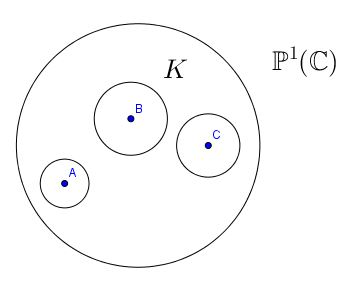
\includegraphics[width=5.7cm]{lezione-161024-fig1}
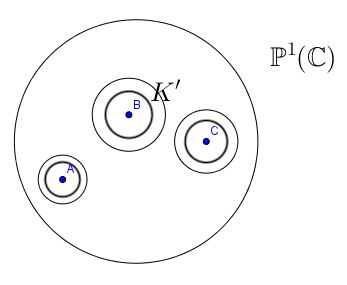
\includegraphics[width=6cm]{lezione-161024-fig2}
\caption{$K$ e $K'$}\label{fig:1}
\end{figure}

Quindi se $A, B, C$ sono i punti che si tolgono da $\mathbb{P}^1(\mathbb{C})$, allora si può scegliere $K'$ come $\mathbb{P}^1(\mathbb{C})\minus\{D_A\cup D_B\cup D_C\}$, con $D_A$ disco aperto attorno a $A$, $D_B$ disco aperto attorno a $B$, $D_C$ disco aperto attorno a $C$, perciò la proprietà.\\
Si osserva che la proprietà $\mathcal{P}$ è invariante per omeomorfismi quindi in particolare per biolomorfismi e che quindi non essendo soddisfatta dalle superfici di Riemann Sferica e Euclidee ne segue che $S$ è iperbolica.
Infatti si ha che si escludono le superfici compatte prendendo come $K'$ loro stesse, si esclude $\bbC$ prendendo come $K'$ il complementare di un disco aperto che contiene $K$ e si esclude $C^*=\mathbb{P}^1(\mathbb{C})\minus\{ 0,\infty\}$ perché con il ragionamento fatto per dimostrare la proprietà $\mathcal{P}$ su $S$ si dimostra che si trovano dei compatti $K'$ con $2$ componenti connesse, quindi non $almeno\hquad 3$, come richiesto dalla proprietà.
\end{itemize}
\end{proof}

\notamargine{La proprietà $\mathcal{P}$ in un qualche senso "conta i punti tolti, in funzione di quello che è rimasto". Inoltre permette di dire per esempio che un "toro meno $n$ punti distinti" non è omeomorfo a un "toro meno $m$ punti distinti", se $m\ne n$}

Possiamo ora usare che $S$ è iperbolica per mostrare l'importante

\begin{teorema}[Teorema di Picard]
Ogni funzione intera ($\bbC\rightarrow\bbC$ olomorfa su tutto $\bbC$) non costante assume tutti i valori tranne al più uno.
\end{teorema}

\begin{osservazione}
\begin{itemize}
\item La mappa esponenziale assume tutti i valori tranne lo $0$
\item Se la mappa $f$ come da ipotesi ha in più la proprietà di NON avere una discontinuità essenziale all'infinito allora si ha che per Liouville deve essere un polinomio, quindi il risultato è banale ($p(x)-a$ ha sempre almeno una radice, se $p$ non costante)
\end{itemize}
\end{osservazione}

\notamargine{C'è anche una versione più forte di questo teorema (detto da lui)}

\begin{proof}
Si usa che $\mathbb{P}^1(\mathbb{C})\minus\{ A, B, C\}$ con $A, B, C$ tre punti distinti è una superficie di Riemann iperbolica (Esercizio 7).\\
Si suppone per assurdo che $f$ soddisfacente le ipotesi non assuma due valori, che a meno di comporre $f$ con un'affinità (automorfismo di $\bbC$) suppongo essere $0,1$.
Allora $f$ induce una mappa olomorfa $f:\bbC->S$ (con $S$ come in Esercizio 7).
Si ha che quindi $f$ si solleva a $\tilde{f}:\bbC\rightarrow D$, con $D$ il disco aperto. DIAGRAMMA \\
Ma allora la mappa olomorfa $\tilde{f}$ è costante per Liouville, quindi poiché il diagramma commuta anche $f$ è costante, assurdo.
\end{proof}

\begin{osservazione}
\begin{itemize}
\item Questo è un teorema non di facile dimostrazione, il punto più delicato nella dimostrazione data è il teorema di Riemann.
\item Nella dimostrazione data il teorema di Riemann serve per l'esistenza di un rivestimento $\pi:D\cong \mathcal{H} \rightarrow S$. In effetti si può dimostrare il teorema di Picard esibendo un rivestimento, Picard face proprio così. Trovò il rivestimento quozientando $\mathcal{H}$ per il gruppo $\Gamma(2)=\{ \frac{az+b}{cz+d} | a,b,c,d\in \bbZ, ad-bc=1, a\cong d \cong 1 \pmod{2}, b\cong c \cong 0 \pmod{2} \}$, dopo aver dimostrato che questo gruppo agiste su $\mathcal{H}$ con le proprietà viste nelle scorse lezioni poiché effettivamente il quoziente sia una superficie di Riemann ed aver verificato che il quoziente è $S$.
\item Ci sono molte altre dimostrazioni con tecniche più analitiche, quella che si è fatta è più geometrica, senza stime.
\end{itemize}
\end{osservazione}

\section{I tori vengono da $\bbC$}
Dato che a noi interesseranno soprattutto i tori, mostriamo questo fatto importante.
\begin{teorema}
    Tutte le strutture complesse di un toro derivano da $\bbC$.
\end{teorema}
\begin{proof}
    Abbiamo visto che l'unica \sdR sferica è $\hat\bbC$; se un toro $T$ fosse sferico, dovrebbe essere biolomorfo a $\hat\bbC$, il che è impossibile ad esempio per questioni di $\pi_1$.

    Quindi dobbiamo cercare un sottogruppo $G<\Aut(\mathcal H)=PSL_2(\bbR)$ senza punti fissi e che agisca in modo propriamente discontinuo, tale che $\mathcal H / G \cong T$.\\
    Osserviamo intanto che vale $\pi_1(T)=\pi_1(\mathcal H / G) = G$ poiché $\mathcal H$ è semplicemente connesso, e quindi $G\cong \bbZ^2$ e in particolare è abeliano.

    Considero $g\in G \setminus \{\Id\}$ e voglio vedere se il centralizzatore di $g$ può contenere uno $\bbZ^2$; posso coniugare tramite un elemento di $PSL_2(\bbR)$ in modo che succeda una delle due cose:
    \begin{enumerate}
        \item $g$ sia una traslazione
        \item $g$ sia un'omotetia
    \end{enumerate}
    Nel caso $1$, $g=g_t=\{z\mapsto z+t\}$ e prendo un $\gamma\in PSL_2(\bbR)$ tale che $\gamma\circ g_t = g_t\circ \gamma$. Valuto l'uguaglianza precedente in $\infty$ e ottengo $\gamma(\infty)=g_t(\gamma(\infty))$, ovvero $\gamma(\infty)=\infty$ dato che $g_t$ è una traslazione. Ma allora vale $\gamma = az+b$, e sostituendo ottengo $a(z+t)+b=az+b+t$, da cui $at=t$ perciò $a=1$.\\
    Dunque il centralizzatore di una traslazione sono le traslazioni, di cui l'unico sottogruppo discreto ha rango $1$.

    Nel caso $2$, prendiamo $g=g_\mu=\{z\mapsto \mu z\}$ e un $\gamma$ che commuta. Valutando in $0$ e $\infty$ otteniamo $\gamma(0)=g_\mu(\gamma(0))$ e $\gamma(\infty)=g_\mu(\gamma(\infty))$.\\
    Dato che gli unici punti fissi di $g_\mu$ sono $0$ e $\infty$, abbiamo due casi possibili:
    \begin{itemize}
        \item $\gamma$ fissa $0$ e $\infty$, quindi è un'omotetia
        \item $\gamma(0)=\infty,\gamma(\infty)=0$ e dunque $\gamma(z)=\frac b \gamma$
    \end{itemize}
    Nel secondo caso $\gamma\not\in\bbZ^2$ perché ha ordine finito. Nel primo caso abbiamo delle omotetie reali, che tramite $\log$ possiamo mandare in un sottogruppo additivo di $\bbR$, che ha rango $1$ se è discreto.

    In conclusione per ogni $g$ il centralizzatore non contiene $\bbZ^2$, quindi non esiste alcun $G$ per cui $\mathcal H / G = T$
\end{proof}
